\chapter{Ionización del medio y simulaciones Monte Carlo}
%%%%%%%%%%%%%%%%%%%%%%%%%%%%%%%%%%%%%%%%%%%%%%%%%%%%%%%%%%%%%%%%%%
%%%%%%%%%%%%%%%%%%%%%%%%%%%%%%%%%%%%%%%%%%%%%%%%%%%%%%%%%%%%%%%%%%
\section{Modelado del fenómeno físico}
\noindent Uno de los aspectos que se propuso estudiar en este trabajo es el de las razones físicas que hacen que el factor de Fano sea un número mucho menor que la unidad, como podría ingenuamente esperarse desde una descripción puramente poissoniana de la interacción.\\
%\indent El factor de Fano del sensor se calcula como el cociente entre la varianza $\sigma^{2}$ de la distribución de carga correspondiente a los eventos de interés y su valor medio $\mu$, como por ejemplo, los picos de los espectros generados por los rayos $X$ del flúor o el aluminio. 
\indent Dado que el proceso de ionización de carga es un proceso estocástico en el cuál un fotón puede o no interactuar con los electrones de la red, este puede pensarse como una serie de experimentos de Bernoulli, donde el \textit{éxito} es ionizar y generar un par electrón hueco y el \textit{fracaso} es no hacerlo. Como la probabilidad de ionización es baja, pero la cantidad de veces que puede darse la interacción es muy alta, en el límite el proceso es poissoniano. Sin embargo, experimentalmente se observa que cuando toda la energía de la partícula incidente es depositada en el material, el factor de Fano resulta casi un orden de magnitud menor\cite{TesisKevin}. Una de las posibles razones por las que esto sucede es que la energía de los fotones incidentes no solo es disipada en forma de ionización de carga, sino también en excitación de fonones de la red cristalina del material.\\
\indent Cuando un fotón de alta energía cinética impacta contra el sensor, este produce una dispersión por ionización y emisión de fonones de la red cristalina del silicio, produciendo así una cascada de pares electrón-hueco. El número de pares producidos puede ser luego medido y el valor de la energía de creación electrón-hueco promediado a partir de este.\\
\indent Este fenómeno es estudiando en los trabajos de R.C. Alig et al.\cite{Alig}, mediante simulaciones de Monte Carlo y luego por K. Ramanathan \cite{Ramanathan}, compilando resultados y propuestas de diferentes trabajos. En el primero se propone un modelo en el que la partícula incidente interactúa con el material, generando pares electrón-hueco por ionización en forma de cascada y, eventualmente, perdiendo energía por emisión de fonones. La forma en que la partícula incidente pierde energía depende fuertemente de la energía que tiene al momento de ionizar. Esta dependencia está modelada en el trabajo de Ramanathan\cite{Ramanathan} y lo llaman \textit{modelo simplificado}, donde proponen que la energía $E$ que se transfiere para generar pares electrón-hueco se reparte según una distribución Beta, de la forma
\begin{equation*}
    p(x|\alpha) = \frac{2}{B(\alpha)} x^{\alpha - 1}(1-x)^{\alpha - 1}
\end{equation*}
donde $x = \frac{E}{E_{r} - E_{g}}$ es la variable aleatoria, con $E_{r}$ la energía inicial de la partícula en cada ionización, $E_{g}$ es la energía del gap del silicio y $E$ la fracción de energía que va a parar a un nuevo par electrón hueco. Utilizando esta distribución para generar realizaciones de la variable aleatoria $x$, se puede despejar el valor de $E$, que es la energía transferida para generar pares electrón-hueco según este modelo. Por otro lado, $B(\alpha)$ es la función Beta con un único parámetro $\alpha$, y viene dada por
\begin{equation*}
    B(\alpha, \beta) 
    = \frac{\Gamma(\alpha)\Gamma(\beta)}{\Gamma(\alpha) + \Gamma(\beta)}
    \longrightarrow
    B(\alpha)
    = \frac{\Gamma^{2}(\alpha)}{2\Gamma(\alpha)}
\end{equation*}
donde $\alpha$ depende de la energía $E_{r}$ y es el parámetro que determina el régimen de distribución de la energía, o en otras palabras, la forma de la distribución.\\
\indent La motivación de la utilización de la distribución Beta para modelar cómo se reparte la energía en la generación de pares electrón-hueco por ionización se debe a que esta se adapta muy bien a los tres tipos de regímenes de energía en los que se puede encontrar la partícula incidente, según los trabajos mencionados anteriormente:
\begin{itemize}
    \item \textbf{A bajas energías de la partícula incidente}, se tienen distribuciones muy picudas en los extremos posibles: $E = 0$ y $E = E_{R}+E_{g}$,
    \item \textbf{A energías mucho mayores que la energía del gap}, $E_{R} >> E_{g}$: Se tiene una distribución aproximadamente uniforme,
    \item \textbf{A energías entre $3.4\,\si{eV}$ - $4.2\,\si{eV}$} se tiene una distribución de energía muy picuda en el medio de $x = E/(E_{R} - E_{g})$.
\end{itemize}
Para energías bajas, el parámetro $\alpha$ tiende a cero y se tiene una distribución con máximos en los extremos del intervalo. Para energías entre $3.4\,\si{eV}$ y $4.2\,\si{eV}$ se tiene una distribución con un máximo en el medio del intervalo y el parámetro $\alpha$ puede tender a infinito. Por último, para energías mucho mayores a la energía del gap, el parámetro $\alpha = 1$ y la distribución es uniforme. Estos casos se resumen en el gráfico de la figura \ref{fig:BetaDist}.\\
\begin{figure}%[H]
% Este gráfico se hace con el script que está acá: /home/igna/Escritorio/Tesis2021/Figs/Figuras_Apendice_Simulaciones/pys_para_plots DistBetaFig.py
    \centering
        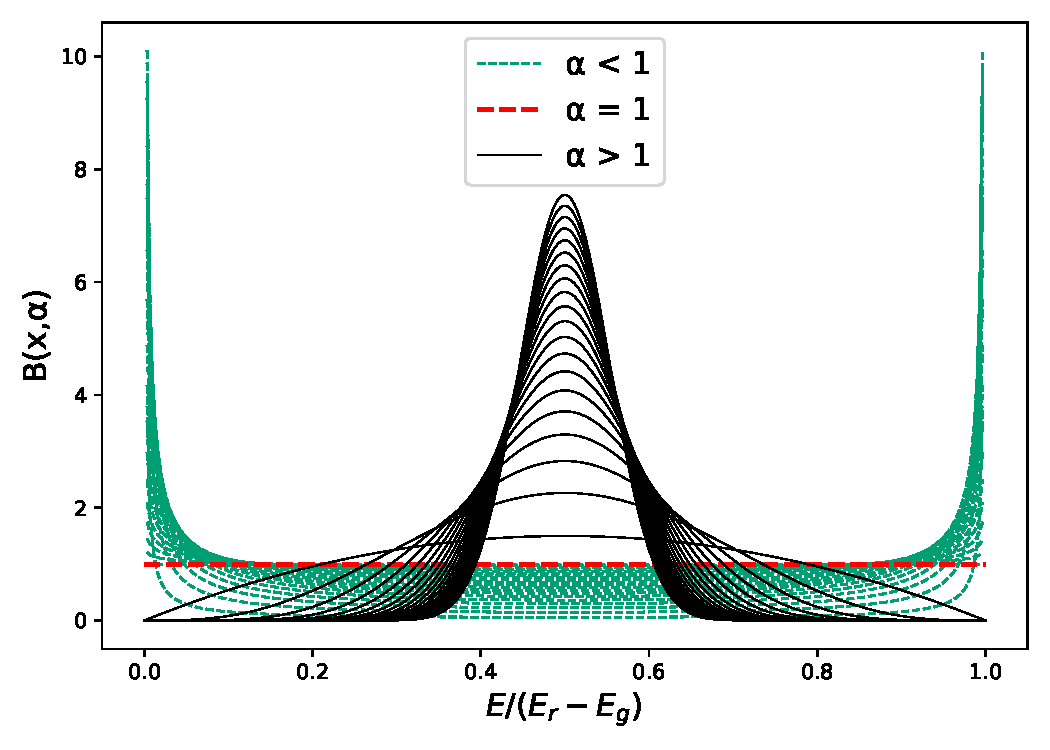
\includegraphics[scale=.7]{Figs/BetaDistFig.pdf}
    \caption{\footnotesize{Distribución Beta para diferentes valores del parámetro $\alpha$}}
    \label{fig:BetaDist}
\end{figure}
\indent El mecanismo de cascada por el cual se producen las ionizaciones consiste en que para una dada energía inicial $E_{R}$, una fracción de esa energía se utiliza para generar un par electrón-hueco y la energía restante vuelve a fraccionarse para generar otros pares electrón-hueco. Estos pares generados, a su vez, utilizan fracciones de esa energía que les fue entregada para generar otros pares, en un proceso que se repite hasta que la energía disponible para repartir en cada rama de la cascada es menor a la energía del gap del Silicio y ya no es suficiente para generar más pares. Durante todo este proceso existe una probabilidad no nula de que parte de la energía se pierda por emisión fonones en la red.\\
\indent Se define una probabilidad $P_{eh}$ para la cual se produce ionización y una probabilidad $1 - P_{eh}$ para la cual se produce emisión de fonones. Esta probabilidad depende de la energía inicial, al igual que el parámetro $\alpha$ de la distribución Beta, y viene dada por
\begin{equation}
    P_{eh}(E_{R}) = 
    \left[
        1 + \frac{\Gamma_{ph}(E_{R})}{\Gamma_{eh}(E_{R})}
    \right]^{-1}
        \label{ec:ProbabilidadIonizacion}
\end{equation}
donde 
\begin{equation*}
    \frac{\Gamma_{ph}(E_{R})}{\Gamma_{eh}(E_{R})}
    = A\frac{105}{2\pi}\frac{(E_{R} - \hbar \omega_{0})^{1/2}}{(E_{R} - E_{g})^{7/2}}
\end{equation*}
con $A = 5.2\,\si{eV^{3}}$, que es una constante fenomenológica que contiene información microscópica del sistema y que además puede ajustarse para reproducir valores medidos experimentalmente. Por otro lado, $\Gamma_{ph}$ y $\Gamma_{eh}$ son las tasas de producción de fonones y pares electrón-hueco, respectivamente.\\
\indent Partiendo de estas ideas, se buscó simular este mecanismo de ionización a partir de simulaciones Monte Carlo.
%%%%%%%%%%%%%%%%%%%%%%%%%%%%%%%%%%%%%%%%%%%%%%%%%%%%%%%%%%%%%%%%%%
%%%%%%%%%%%%%%%%%%%%%%%%%%%%%%%%%%%%%%%%%%%%%%%%%%%%%%%%%%%%%%%%%%
\section{Simulaciones básicas}
\noindent El modelo más simplificado del mecanismo de ionización puede pensarse como una serie de experimentos de Bernoulli, es decir, donde solo hay dos resultados posibles: éxito-fracaso. Donde la probabilidad de éxito $p$, que es la probabilidad de ionizar una carga y perder una cantidad de energía equivalente a la energía de creación electrón-hueco del silicio, sin tener en cuenta de ninguna forma la disipación de energía por excitación de fonones.\\
\indent Dada una energía inicial y un número fijo $N$ de experimentos de Bernoulli, puede suceder que la energía inicial se agote completamente o no. El valor final de la energía depende muy fuertemente del valor de $N$: Para una cantidad de experimentos $N$ muy grande, la probabilidad de que la energía se agote completamente tiende a $1$, mientras que para $N$ muy pequeño la probabilidad es mucho menor, pudiendo suceder que la energía no sea cero al final del experimento. No es sorprendente que con este modelo se recupera un factor de Fano que tiende a $1$, en el caso en el que el valor de $N$ es grande pero no suficiente para agotar la energía de la partícula incidente. Esto es debido a que la realización de experimentos consecutivos de Bernoulli conforman una variable aleatoria de distribución binomial, la cual tiende a una distribución de Poisson si además $p$ es pequeño. Esto puede verse en la figura \ref{fig:SimulacionOrden0Fano1}, donde claramente puede verse que una distribución Poissoniana ajusta muy bien al histograma. Esta corresponde a una simulación que parte de una energía inicial de $677\,\si{eV}$ con un $N = 5000$, que es la cantidad de veces que se repite el experimento de Bernoulli de ionizar o no con probabilidad $p=0.01$ y el factor de Fano resultó $F = 0.991$. A su vez, este experimento se repitió $20000$ veces para tener una buena cantidad de estadística para formar el histograma.\\
\begin{figure}%[H]
%Para hacer este gráfico hay que correr el script que está en esta carpeta /home/igna/Escritorio/Tesis2021/Figs/Figuras_Apendice_Simulaciones/pys_para_plots y se llama Orden0_simu_SI_atraviesa.py con los datos de esta carpeta /home/igna/Escritorio/Tesis2021/Figs/Figuras_Apendice_Simulaciones/txts_para_plots y se llama orden0_simu_SI_atraviesa.txt
    \centering
    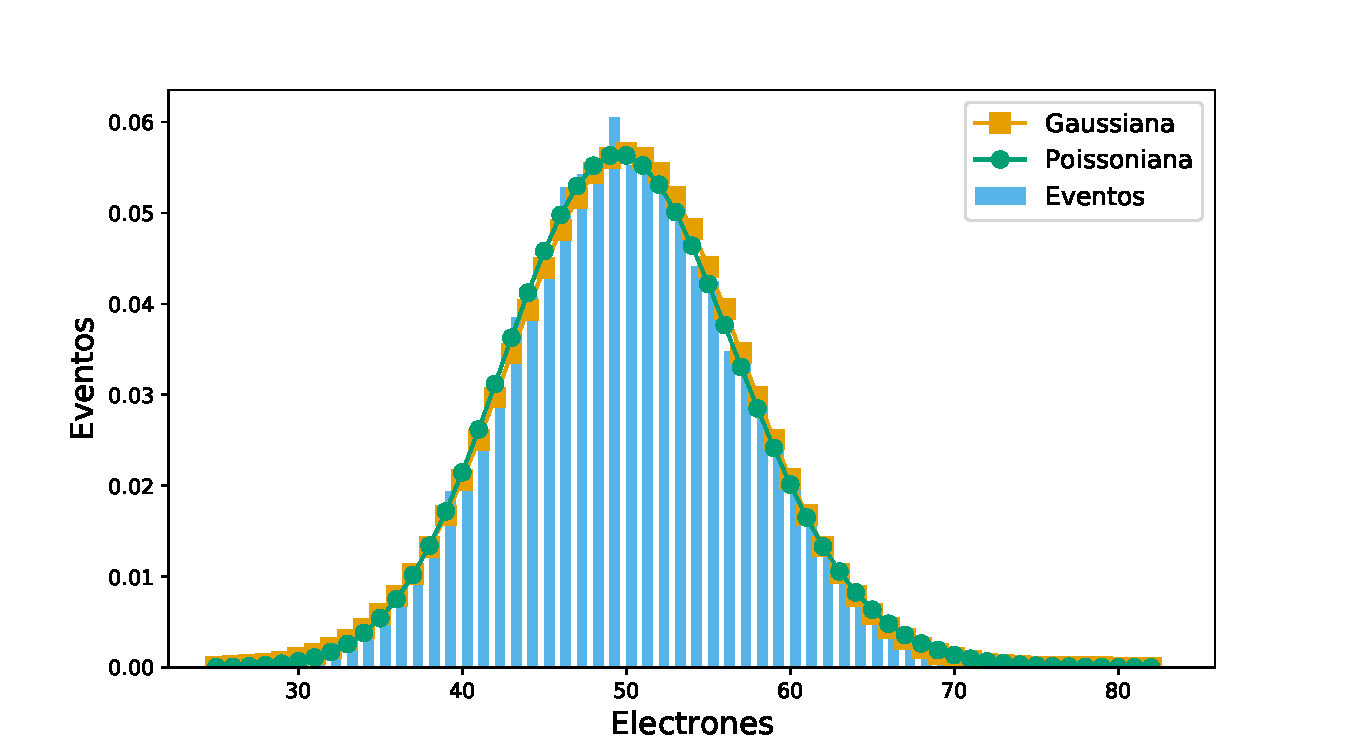
\includegraphics[scale=0.35]{Figs/Orden0_fano1.pdf}
    \caption{\footnotesize{Histograma, con los correspondientes ajustes, Gaussiano y Poissoniano, de los resultados de $2\times 10^3$ experimentos, cada uno de los cuales consiste de $N = 5000$ experimentos de Bernoulli. En este caso la energía final de la partícula no es cero, es decir, la partícula incidente logra atravesar el material. Puede verse como el ajuste poissoniano ajusta muy bien al histograma.}}
    \label{fig:SimulacionOrden0Fano1}
\end{figure}
\indent Por el contrario, para el caso en que $N$ es tal que la gran mayoría de las veces la energía se agota completamente, el factor de Fano se vuelve menor a $1$, como puede verse en la figura \ref{fig:SimulacionOrden0Fano0}. En este caso, nuevamente se parte de una energía inicial de $677\,\si{eV}$ pero esta vez con un $N = 30000$, cantidad suficiente para agotar completamente la energía y $p=0.01$ nuevamente. Se repitió $20000$ veces el experimento para obtener una buena cantidad de estadística para formar el histograma. En este caso el factor de Fano fue de $F = 0.297$.\\
\begin{figure}%[h]
%Para hacer este gráfico hay que correr el script que está en esta carpeta /home/igna/Escritorio/Tesis2021/Figs/Figuras_Apendice_Simulaciones/pys_para_plots y se llama Orden0_simu_NO_atraviesa.py con los datos de esta carpeta /home/igna/Escritorio/Tesis2021/Figs/Figuras_Apendice_Simulaciones/txts_para_plots y se llama orden0_simu_NO_atraviesa.txt
    \centering
    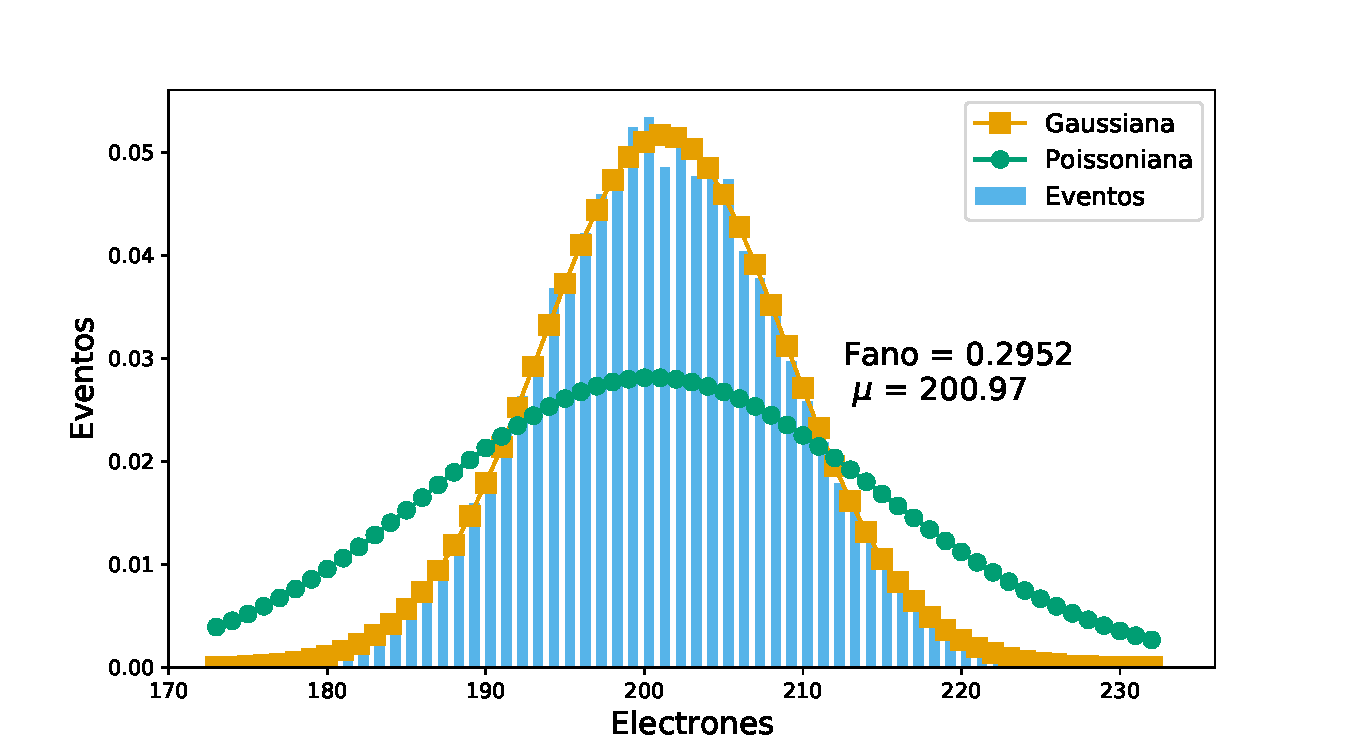
\includegraphics[scale=0.35]{Figs/Orden0_fano0.pdf}
    \caption{\footnotesize{Histograma, con los correspondientes ajustes, Gaussiano y Poissoniano, de los resultados de $2\times 10^3$ experimentos, cada uno de los cuales consiste de $N = 30000$ experimentos de Bernoulli. En este caso la energía final de la partícula es casi siempre cero, es decir, la partícula incidente pierde toda su energía dentro del material. Es en este caso en el que el factor de Fano da menor a la unidad.}}
    \label{fig:SimulacionOrden0Fano0}
\end{figure}
\indent Si bien este modelo de juguete es una simplificación del proceso de dispersión real, los resultados están en concordancia con la hipótesis de que el factor de Fano es menor a $1$ debido a que la partícula incidente deposita toda su energía en el material.\\
%%%%%%%%%%%%%%%%%%%%%%%%%%%%%%%%%%%%%%%%%%%%%%%%%%%%%%%%%%%%%%%%%%
%%%%%%%%%%%%%%%%%%%%%%%%%%%%%%%%%%%%%%%%%%%%%%%%%%%%%%%%%%%%%%%%%%
\section{Simulación de ionización en cascada}
\noindent Utilizando ideas tomadas de los trabajos anteriormente citados, se modificaron las simulaciones Monte Carlo con la intención de reproducir el mecanismo de creación de pares electrón-hueco por ionización en cascada. Para este caso se tuvo en cuenta la posibilidad de disipación de energía por emisión de fonones, a una energía fija de $\hbar\omega_{0} = 0.063\,eV$.\\
\indent El resultado de la simulación es simplemente el número de pares 
ionizados a partir de la energía inicial $E_{R}$. De esta puede verse la distribución de la cantidad de pares generados y además calcular tanto su varianza como su esperanza, para así obtener el factor de Fano.\\
\indent Otro elemento a tener en cuenta en la simulación es la conservación de la energía durante el proceso de creación de pares. Puede considerarse que la energía transferida al ionizar es utilizada totalmente para ionizar otros pares o puede considerarse que siempre que se de una ionización habrá una pequeña parte de energía que se pierde y no puede ser utilizada, es decir, que no se conserva la energía. Cabe destacar que en este tipo de simulación, dada su implementación particular, solo se puede considerar el caso en que la partícula disipa toda su energía en el interior del material, de modo que se esperan valores para el factor de Fano menores a la unidad.\\
\indent Se realizaron las simulaciones partiendo de una energía inicial $E_{r} = 677\,\si{eV}$, correspondiente a los rayos $X$ de flúor, que es el principal objeto de estudio de este trabajo. Los valores de los parámetros fueron extraídos de la bibliografía\cite{Alig}\cite{Ramanathan} y son $A = 5.2\,\si{eV}^{3}$, la energía del gap $E_{g} = 1.1\,\si{eV}$, la energía de creación electrón-hueco promedio $\varepsilon_{eh} = 3.75\,\si{eV}$ y la energía perdida cada vez que se emiten fonones $\hbar \omega = 0.063\,\si{eV}$. El resto de los parámetros son configurables y se variaron para ver los diferentes resultados de la simulación, como ser la pérdida de energía al ionizar $E_{loss}$ y la cantidad de repeticiones del experimento. La simulaciones se efectuaron con no menos de $5000$ repeticiones y con diferentes valores de $E_{loss}$.\\
\indent Se simuló el proceso de cascada con con diferente cantidad de repeticiones, partiendo desde $5000$ hasta incluso $100000$ para asegurar la robustez de la estadística. En la figura \ref{fig:FanoConvergencia} se observa la convergencia de los valores del factor de Fano a medida que aumenta el número de experimentos. 
\begin{figure}%[h]
%Este gráfico se puede hacer con el script GrafFanoConvergencia.py que esta en este directorio /home/igna/Escritorio/Tesis2021/Figs/Figuras_Apendice_Simulaciones/pys_para_plots
    \centering
    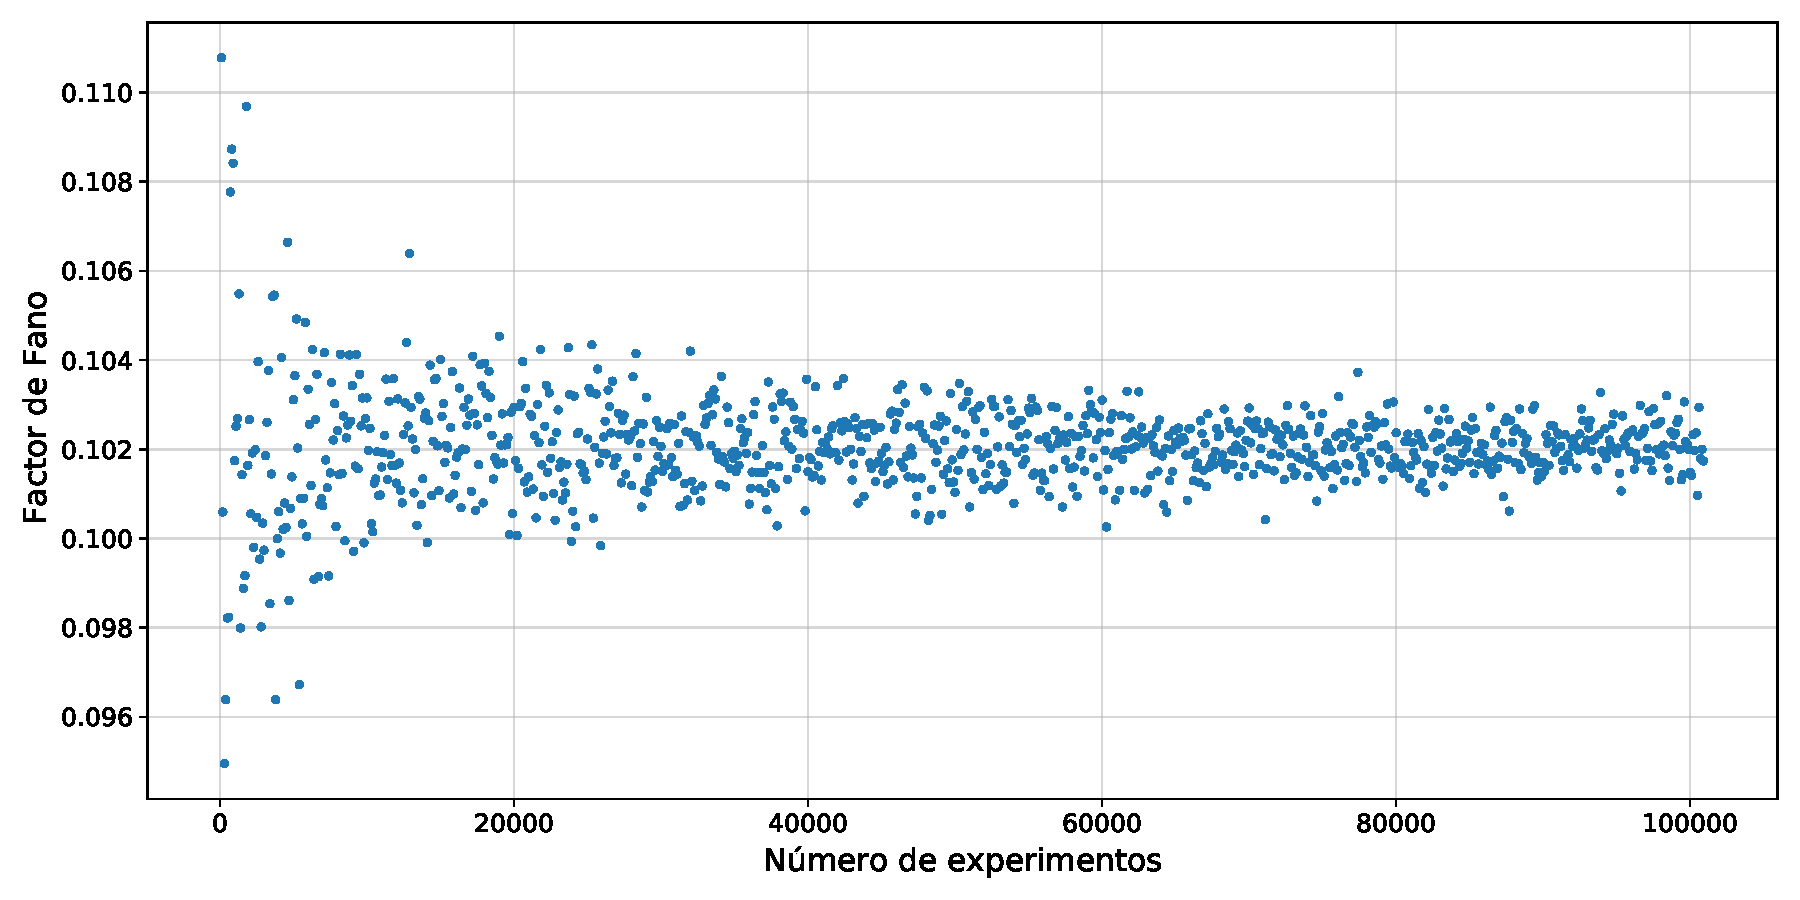
\includegraphics[scale=0.5]{Figs/FanoConvergencia.pdf}
    \caption{\footnotesize{Dispersión de los valores del Factor de Fano cada cantidad de repeticiones del experimento, partiendo desde $100$ repeticiones hasta 100900 repeticiones.}}
    \label{fig:FanoConvergencia}
\end{figure}
Para $10^{4}$ repeticiones se ve que los valores del factor de Fano están acotados entre $\sim 0.106$ y $\sim 0.098$, mientras que para $10^{5}$ repeticiones están acotados entre $\sim 0.100$ y $\sim 0.104$. Se nota claramente la mejora en la estadística.\\
\indent Además, con el fin de poder caracterizar mejor las dependencias entre parámetros en la simulación, se hicieron barridos sobre la pérdida de energía $E_{loss}$ para conocer la dependencia de los resultados respecto de este, partiendo desde $0\,\si{eV}$ de pérdida de energía hasta $7\,\si{eV}$ de pérdida de energía por cada ionización (equivale a perder casi $4$ veces la energía del gap del silicio). En cada uno se midió el factor de Fano, el valor medio de carga ionizada y la energía de creación electrón hueco, como puede verse en las figuras \ref{fig:FanoVsEloss} \ref{fig:ElossVsMu} y \ref{fig:CreacionHuecoVsEloss}. 
\begin{figure}%[h]
%a) Esta figura se puede hacer con los datos de: fano_Eloss_mu_vec.txt que está en el directorio /home/igna/Escritorio/Tesis2021/Figs/Figuras_Apendice_Simulaciones/txts_para_plots usando el .py Barridos_mu_Eloss_fano.py que está en /home/igna/Escritorio/Tesis2021/Figs/Figuras_Apendice_Simulaciones/pys_para_plots
    \centering
    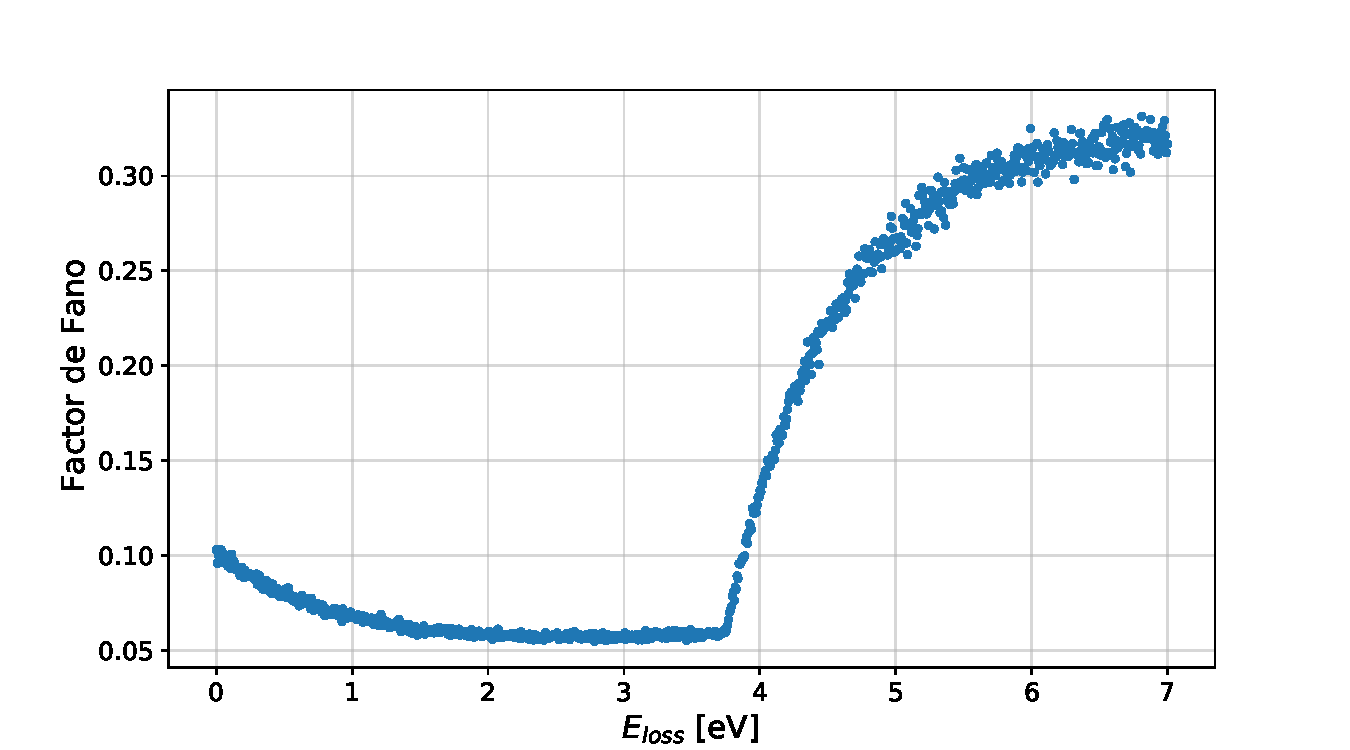
\includegraphics[scale=0.35]{Figs/Fano_vs_Eloss_5ktrials_0-7Eloss.pdf}
    \caption{\footnotesize{Curva del factor de Fano en función de la energía pérdida por cada ionización. El cambio abrupto en la curva ocurre para $E_{loss} = 3.75\,si{eV}$, coincidente con la energía media de creación electrón-hueco.}}
    \label{fig:FanoVsEloss}
\end{figure}
La curva del factor de Fano en función de la energía $E_{loss}$ (y al igual que la energía de creación electrón-hueco y el valor medio de carga ionizada) presenta un cambio de régimen abrupto cuando se cruza el umbral $E_{loss} = 3.75\,\si{eV}$. En la figura \ref{fig:FanoVsEloss} puede verse claramente este cambio de régimen. También se observa que cuando hay conservación de la energía, es decir, $E_{loss} = 0$, es cuando se obtiene un factor de Fano más semejante al observado experimentalmente, que está cerca de $0.1$. A medida que aumenta la pérdida de energía, el factor de Fano comienza a decrecer hasta que se alcanza los $3.75\,\si{eV}$ de pérdida de energía, donde se observa el cambio brusco en la curva, y se observa un aumento pronunciado de la pendiente, semejante a un punto crítico.\\
\indent De la misma forma, el valor medio $\mu$ de la carga ionizada tiene un cambio de concavidad en la curva a medida que aumenta la cantidad de energía perdida por cada ionización, como se ve en la figura \ref{fig:ElossVsMu}.
\begin{figure}%[h]
% b) Esta figura se puede hacer con los datos de: fano_Eloss_mu_vec.txt que está en el directorio /home/igna/Escritorio/Tesis2021/Figs/Figuras_Apendice_Simulaciones/txts_para_plots usando el .py Barridos_mu_Eloss_fano.py que está en /home/igna/Escritorio/Tesis2021/Figs/Figuras_Apendice_Simulaciones/pys_para_plots
    \centering
    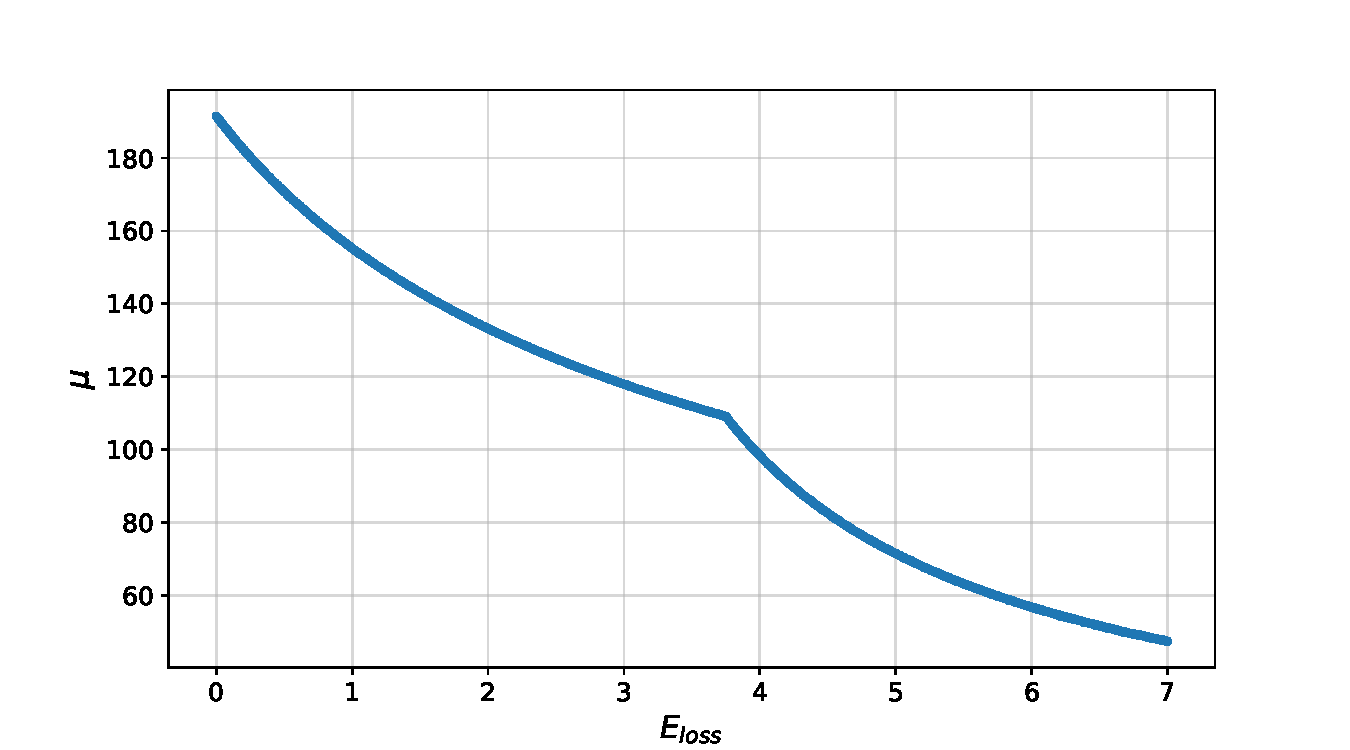
\includegraphics[scale=0.35]{Figs/ELoss_vs_mu_5ktrials_0-7Eloss.pdf}
    \caption{\footnotesize{Curva del valor medio de carga $\mu$ en función de la energía pérdida por cada ionización. El cambio abrupto en la curva ocurre para $E_{loss} = 3.75\,si{eV}$, coincidente con la energía media de creación electrón-hueco.}}
    \label{fig:ElossVsMu}
\end{figure}
Nuevamente, los valores más cercanos a los medidos experimentalmente son los que corresponden a los casos en los que no hay disipación de energía.\\
\indent Por último, para la energía de creación electrón hueco, calculada a partir del valor medio de carga ionizada y la energía inicial $E_{R} = 677\,\si{eV}$, usando $\left\langle\varepsilon_{\eh} \right\rangle= 677\,\si{eV}/\mu$, claramente tendrá el mismo cambio de régimen en $3.75\,\si{eV}$, como se ve en la figura \ref{fig:CreacionHuecoVsEloss}.\\
\begin{figure}%[h]
%a) Esta figura se puede hacer con los datos de: fano_Eloss_mu_vec.txt que está en el directorio /home/igna/Escritorio/Tesis2021/Figs/Figuras_Apendice_Simulaciones/txts_para_plots usando el .py Barridos_mu_Eloss_fano.py que está en /home/igna/Escritorio/Tesis2021/Figs/Figuras_Apendice_Simulaciones/pys_para_plots
    \centering
    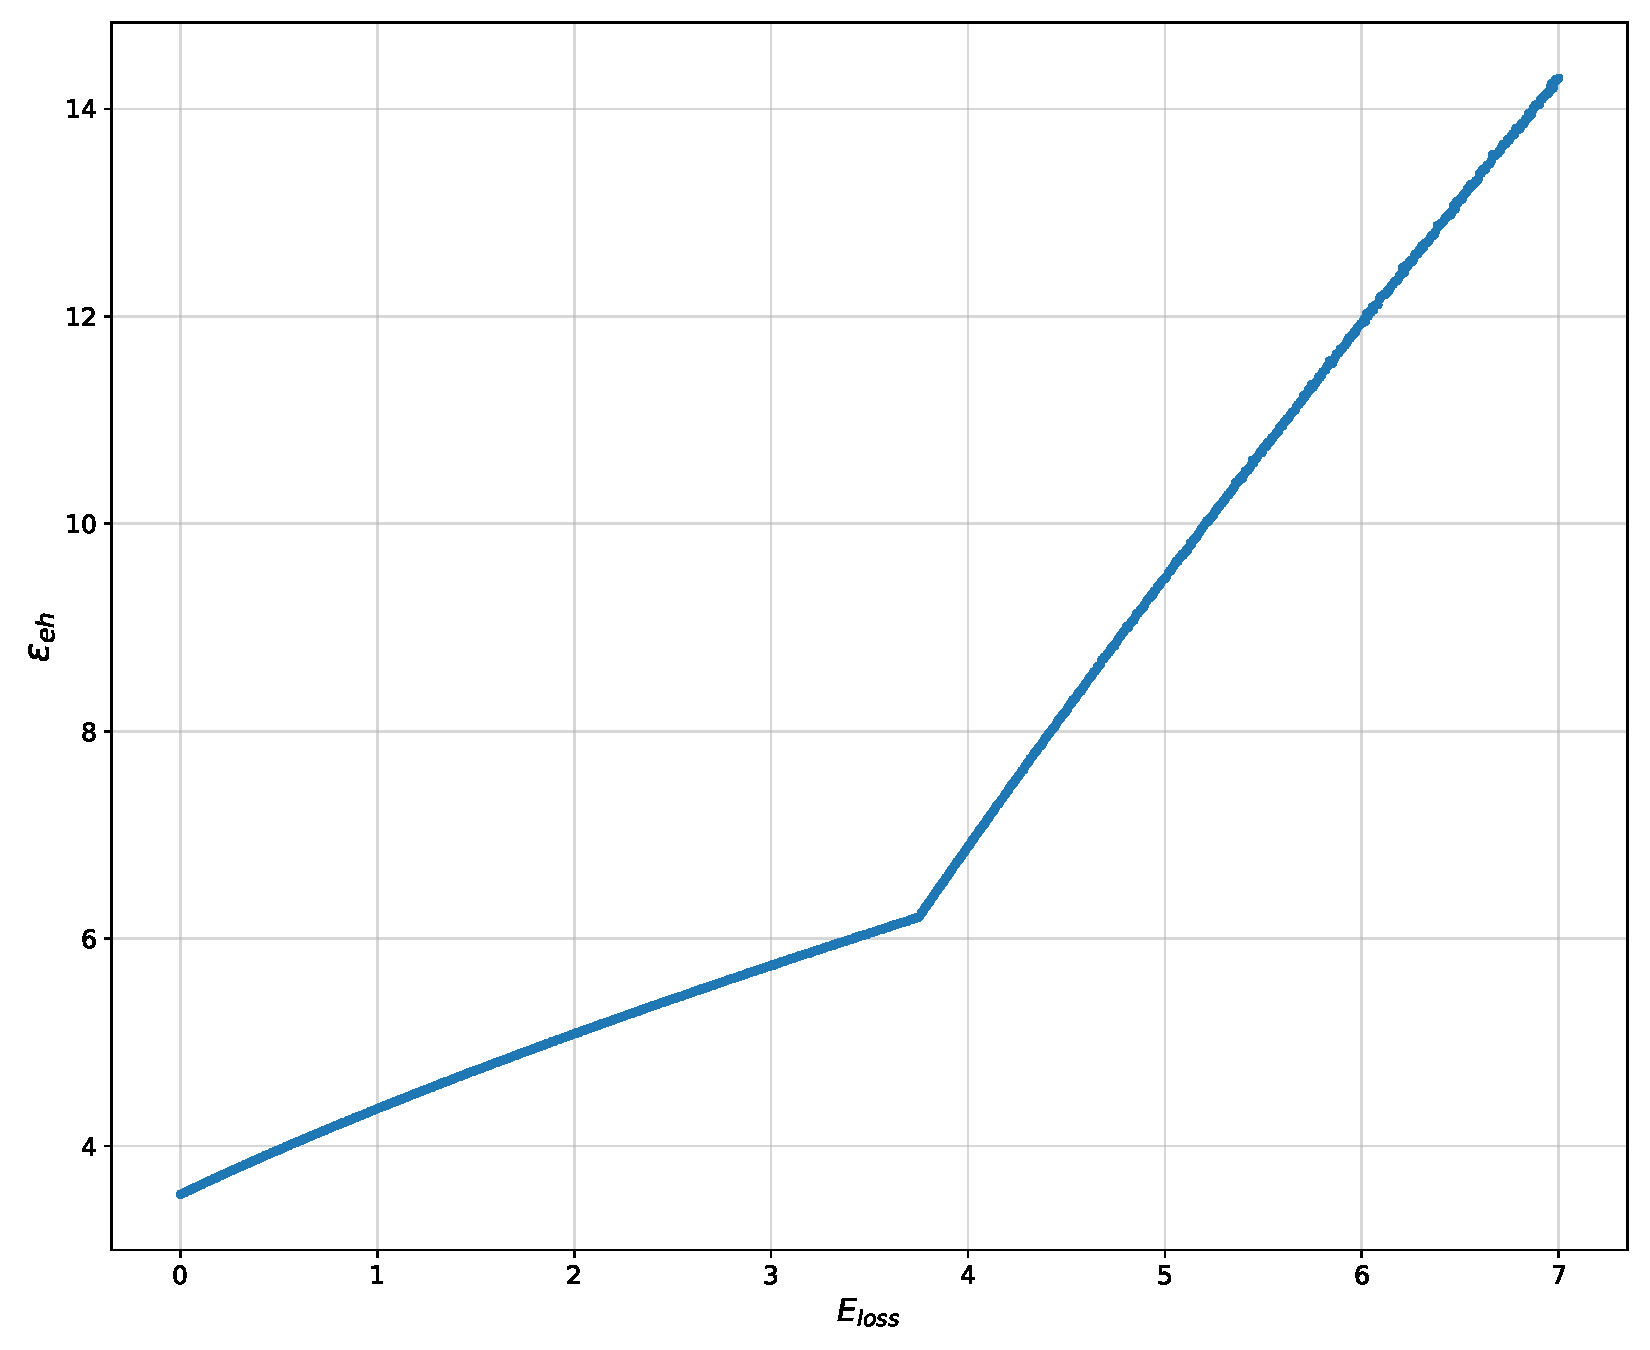
\includegraphics[scale=0.35]{Figs/E_eh_vs_Eloss_5ktrials_0-7Eloss.pdf}
    \caption{\footnotesize{Curva del valor medio de la energía de creación de electrón-hueco en función de la energía pérdida por cada ionización. El cambio abrupto en la curva ocurre para $E_{loss} = 3.75\,si{eV}$, coincidente con la energía media de creación electrón-hueco. Esta curva se obtiene utilizando el valor medio de carga ionizada $\mu$ y la energía inicial $677\,\si{eV}$.}}
    \label{fig:CreacionHuecoVsEloss}
\end{figure}
%Con lo cual se observa que este Monte Carlo es muy sensible a dos parámetros muy importantes de la física real del sistema: La energía de creación electrón hueco, que es el parámetro de la simulación que determina si hay o no ionización\footnote{Como se verá en el apéndice}; y la conservación de la energía.%Se observa que cuando la energía se conserva en la simulación, se obtienen los resultados más cercanos a los observados experimentalmente y reportados en la bibliografía.
\indent Con estos barridos se vio la dependencia de tanto del factor de Fano, como de la energía de creación electrón-hueco y del valor medio de carga ionizada al variar el valor de la energía que se pierde con cada ionización. Se observó que estos parámetros son muy sensibles a la pérdida de energía del sistema, obteniéndose resultados con cambios de regímenes muy pronunciados, particularmente, cuando la energía perdida por ionización coincide con el valor $E_{loss} = 3.75\,\si{eV}$, que casualmente es la energía de creación electrón-hueco promedio y que se usó en la simulación como un parámetro fijo dentro del código\footnote{ver apéndice}.\\
\indent Los resultados de las simulaciones del factor de Fano se ven en los gráficos de las figuras \ref{fig:Simulacion1rden1Fano1} y \ref{fig:Simulacion1rden1Fano2}. Ambos muestran la distribución de carga simulada, un ajuste Gaussiano a ese histograma, usando el $\mu$ y el $\sigma$ generado a partir de los datos y a su vez la forma de la Poissoniana que corresponde a ese valor medio $\mu$. Se ve claramente como la distribución de carga está lejos de parecerse a una distribución de Poisson y por ello el factor de Fano se aleja de la unidad.\\
\indent El primer caso corresponde a una simulación en la que se repitió el mismo experimento de cascada $100000$ veces para tener una buena robustez estadística, mientras que en el segundo caso se usaron $10000$ repeticiones del experimento.\\
\indent En la figura \ref{fig:Simulacion1rden1Fano1} se puede ver lo bien que se ajusta una distribución Gaussiana al histograma. En este caso el factor de Fano correspone a $F = 0.1021$ y el valor medio de carga $\mu = 192 \pm 4$, un valor significativamente mayor que el valor esperado, cercano a $\mu = 181$.
\begin{figure}%[h]
%Los datos para este gráfico están en /home/igna/Escritorio/Tesis2021/Figs/Figuras_Apendice_Simulaciones/txts_para_plots Distribucion_carga_simulada_100k.txt Para modificar el graf hay que correr el .py que están en /home/igna/Escritorio/Tesis2021/Figs/Figuras_Apendice_Simulaciones/pys_para_plots Fano_100k_dist_carga.py
    \centering
\textit{}    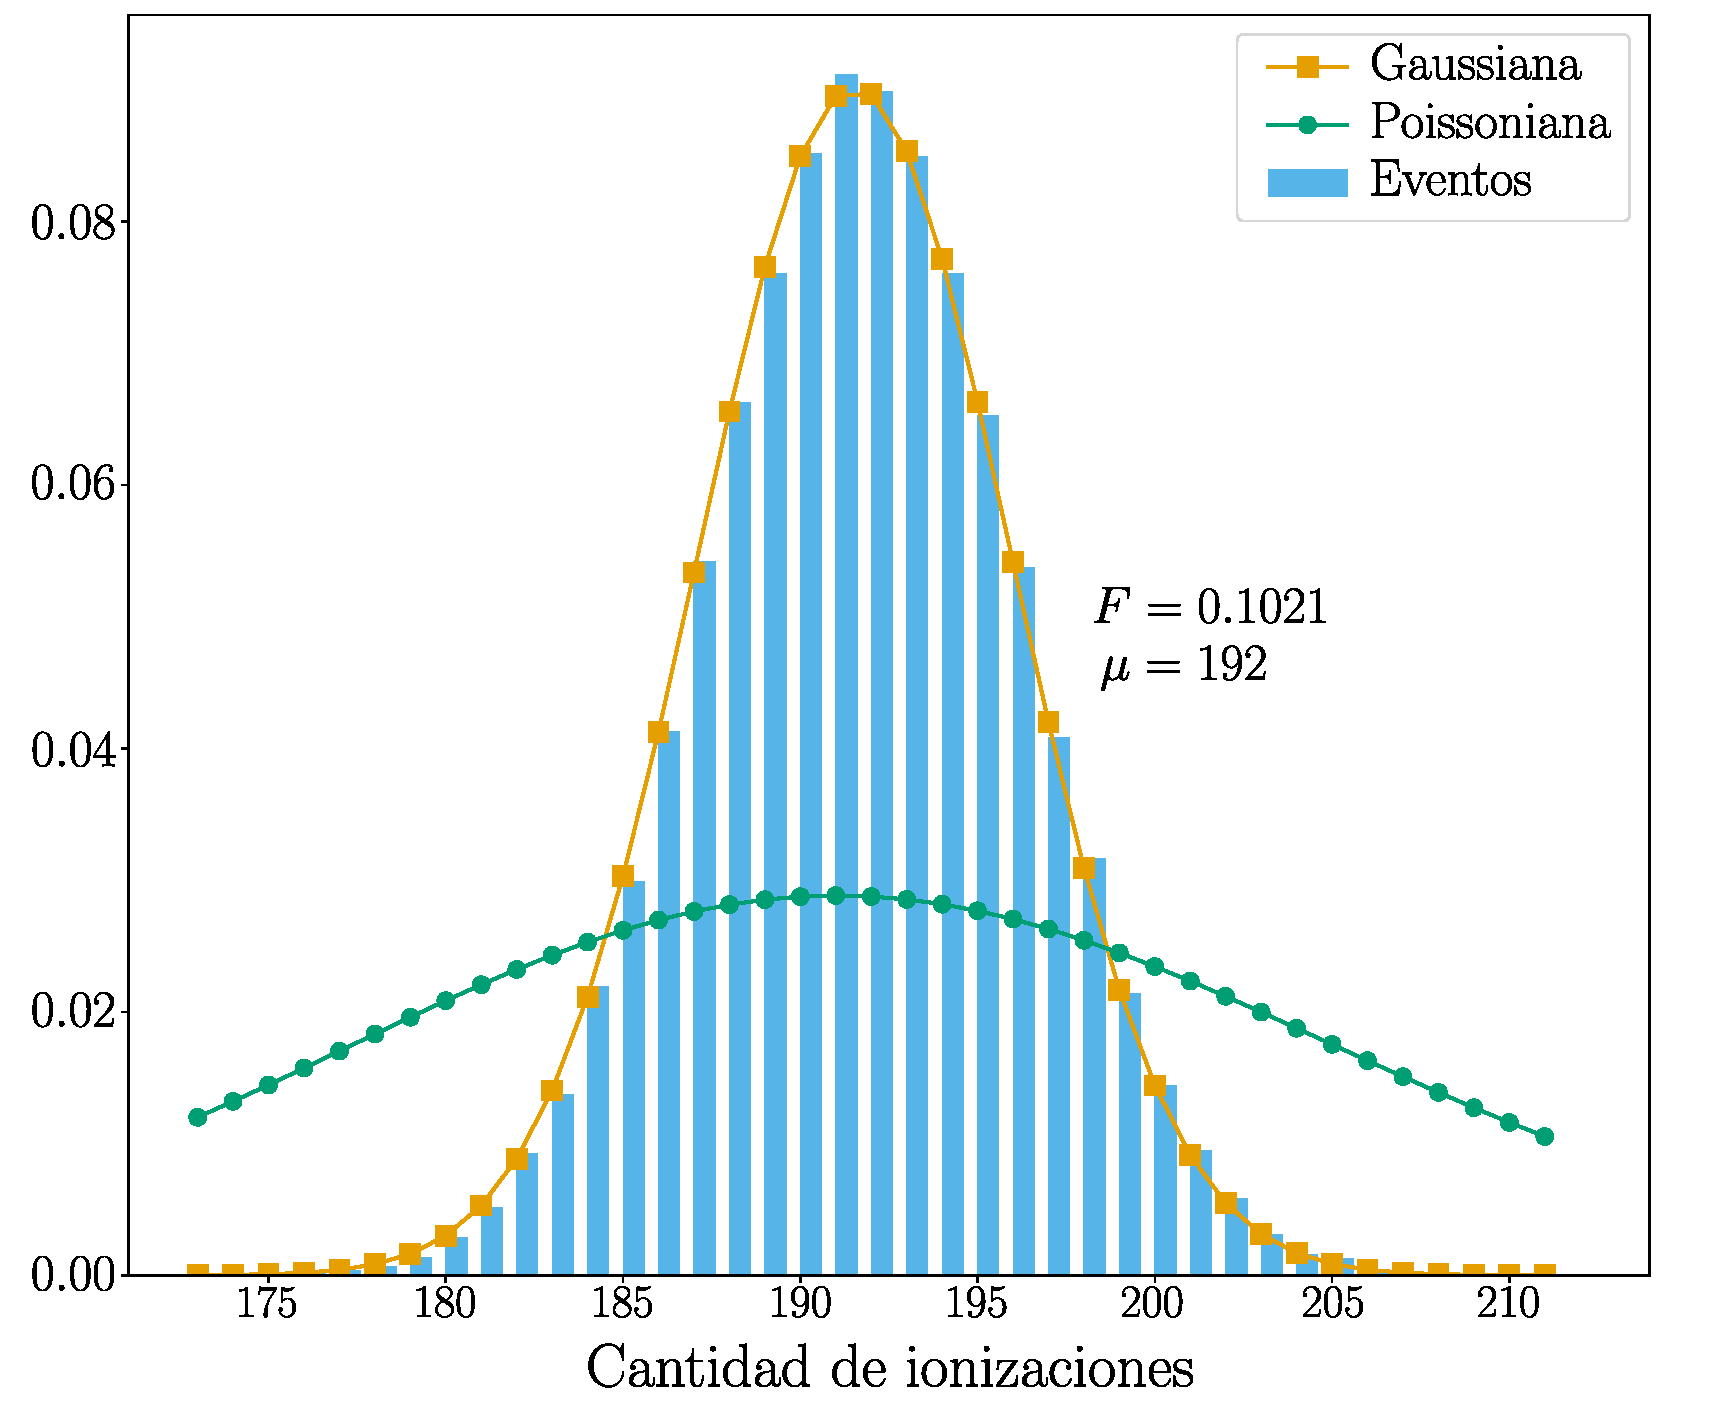
\includegraphics[scale=0.35]{Figs/Fano_677_Eloss0_100ktrials.pdf}
    \caption{\footnotesize{Distribución de carga simulada con el método de Monte Carlo, con parámetro $A = 5.2\,\si{eV}^{3}$ y $100000$ \textit{trials} para obtener la mejor estadística posible. Se observa un valor medio $\mu = 192$, lo cual representa un corrimiento hacia la derecha del valor esperado para el pico de los rayos $X$ del Flúor, que es al rededor de $181$ electrones.}}
    \label{fig:Simulacion1rden1Fano1}
\end{figure}
\noindent Para el segundo caso, en la figura \ref{fig:Simulacion1rden1Fano2}, se modificó el valor del parámetro $A$ de forma que el pico coincida con lo esperado, que son $\mu = 181$ electrones. El valor de $A$ que cumple esa condición es $A = 20\,\si{eV}^{3}$, valor $5$ veces mayor al propuesto en la bibliografía para describir macroscópicamente las propiedades del silicio.
\begin{figure}%[h]
%Los datos para este gráfico están en /home/igna/Escritorio/Tesis2021/Figs/Figuras_Apendice_Simulaciones/txts_para_plots Distribucion_carga_simulada_10k.txt Para modificar el graf hay que correr el .py que están en /home/igna/Escritorio/Tesis2021/Figs/Figuras_Apendice_Simulaciones/pys_para_plots Fano_10k_dist_carga.py
    \centering
    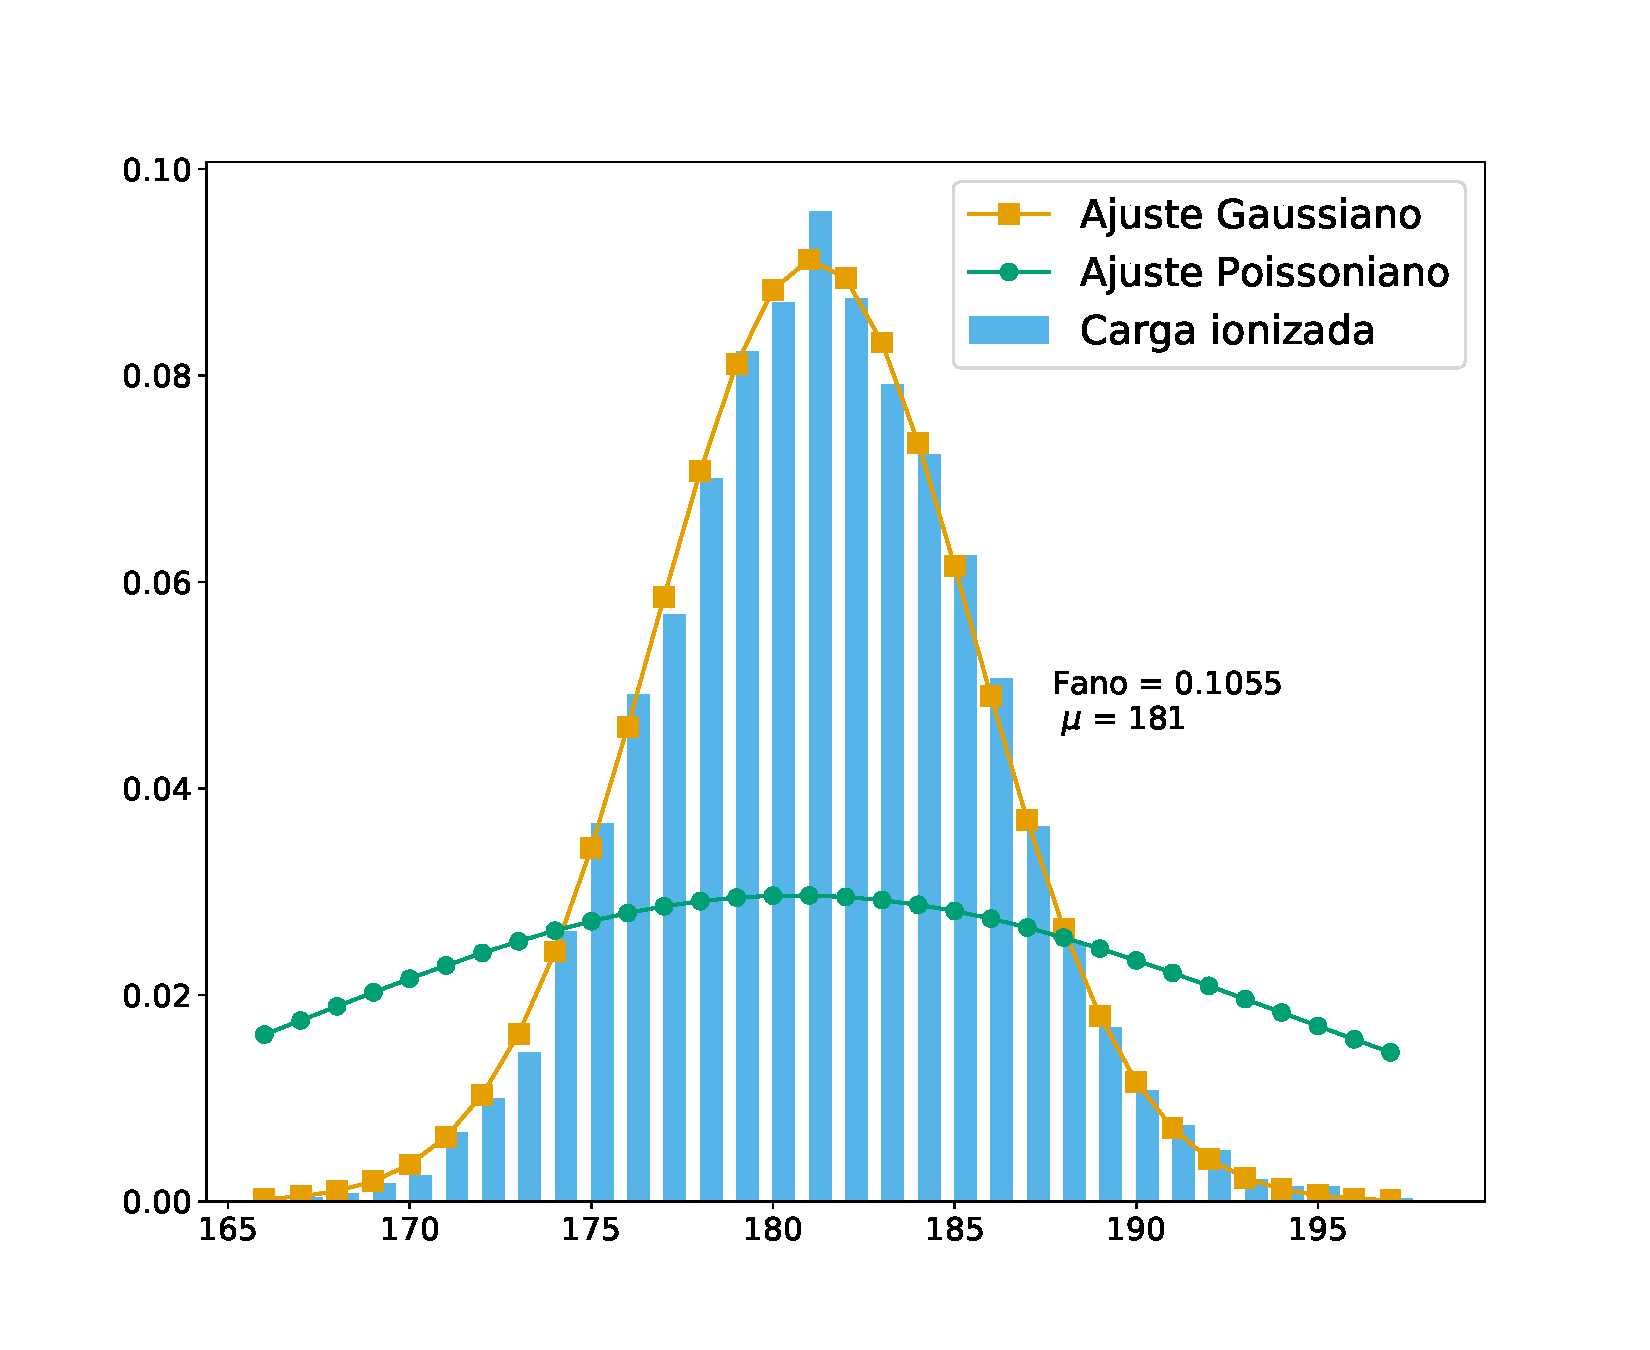
\includegraphics[scale=0.35]{Figs/Fano_677_Eloss0_10ktrials.pdf}
    \caption{\footnotesize{Distribución de carga simulada con el método de Monte Carlo, forzando el parámetro $A$ para que el pico se encuentre en los $181$ electrones esperados para los $677\,\si{eV}$ de energía de los rayos X del Flúor. En este caso $A=20$ y se usaron solamente $10000$ \textit{trials}.}}
    \label{fig:Simulacion1rden1Fano2}
\end{figure}
El factor de Fano en este caso es de $F = 0.1055$, que está contenido entre las bandas esperadas para la cantidad de estadística utilizada en esta simulación.\\%La razón por la cual usar menor estadística en este caso fue porque no era necesaria tanta robustez.\\
\indent En ambos casos el valor del factor de Fano es muy semejante y resulta, como se esperaba, alrededor de un orden de magnitud inferior a la unidad. Los valores esperados son << buscar valores esperados >>.\\
\indent De estas simulaciones se esperaba poder comprender mejor una de las posibles razones de por qué el factor de Fano es menor a la unidad en las mediciones experimentales. La hipótesis que sustentan las simulaciones es que el proceso pierde su carácter Poissoniano al depositar toda su energía en el interior del material, debido a ionización, emisión de fonones y otras pérdidas de energía.
